\\documentclass[11pt]{article}

% ---------- Packages ----------
\\usepackage[margin=1in]{geometry}
\\usepackage[T1]{fontenc}
\\usepackage[utf8]{inputenc}
\\usepackage{lmodern}
\\usepackage{microtype}
\\usepackage{setspace}
\\usepackage{graphicx}
\\usepackage{booktabs}
\\usepackage{multirow}
\\usepackage{array}
\\usepackage{amsmath,amssymb}
\\usepackage[hypertexnames=false]{hyperref}
\\usepackage[nameinlink,noabbrev]{cleveref}
\\usepackage{enumitem}
\\usepackage{float}
\\graphicspath{{figures/}}

% ---------- Formatting ----------
\\onehalfspacing
\\setlength{\\parskip}{0.5em}
\\setlength{\\parindent}{0pt}

% ---------- Metadata ----------
\\title{From Bounded Multimodal Gain to Selective Activation: Gain-Threshold Routing on OpenBG-IMG}
\\author{
Author One\\textsuperscript{1} \\and
Author Two\\textsuperscript{1} \\and
Author Three\\textsuperscript{2}
}
\\date{}

% Running title (copy into target journal template later)
\\newcommand{\\runningtitle}{Selective Multimodal Activation on OpenBG-IMG}

\\begin{document}

\\maketitle

\\begin{center}
\\textsuperscript{1} Department / School / University, City, Country \\\\
\\textsuperscript{2} Department / School / University, City, Country \\\\
\\vspace{0.5em}
\\textbf{Corresponding author:} Author Name \\\\
\\textbf{Email:} \\texttt{corresponding.author@email.com}
\\end{center}

\\begin{abstract}
Multimodal knowledge graph completion (MMKGC) aims to improve link prediction by incorporating auxiliary modalities such as text and images. In product-oriented knowledge graphs, however, visual support is often incomplete, so multimodal evidence does not help uniformly. The key problem is therefore not only whether multimodal information is useful, but when it should be activated under a protocol-shaped missing-modality setting.

We investigate this problem on OpenBG-IMG under a unified protocol with filtered ranking, \\texttt{direction=both}, and three-seed reporting. First, we provide a protocol-aware analysis of the current split and show that role--modality asymmetry entangles target position with image availability: head-side targets may be image-available, whereas tail-side targets are effectively image-unavailable. This reveals a bounded-gain structure in which multimodal benefit is strongest in image-supported head-side regimes but remains limited at the global level.

Second, we propose a gain-threshold routing framework for selective multimodal activation. The framework uses \\texttt{Gate-only} as a fusion expert and \\texttt{Residual-only} as a structural expert, constructs development-side query-level gain labels from reciprocal-rank improvement, and learns a protocol-aware router with target-regime, relation-prior, modality-consistency, and expert-confidence features. A hard threshold is then used to decide whether the current query should activate the multimodal path or fall back to the structural expert.

Experimental results show that the proposed method is effective under the unified query-level routing line. The best learned router (XGBoost with $\\delta=0.01$ and $\\tau=0.7$) reaches an MRR of \\texttt{0.3160}, outperforming \\texttt{Residual-only} (\\texttt{0.2930}), rule-based routing (\\texttt{0.2939}), and the original \\texttt{Full Model} (\\texttt{0.2100}), while Oracle routing (\\texttt{0.3337}) still indicates additional headroom. These results indicate two main contributions of this work: (1) a protocol-aware analysis that reveals the bounded and query-dependent nature of multimodal gain in OpenBG-IMG; and (2) a gain-threshold routing method that converts bounded gain into effective selective multimodal activation.
\\end{abstract}

\\textbf{Keywords:} multimodal knowledge graph completion; selective activation; routing; incomplete visual modality; protocol-aware evaluation

\\section{Introduction}
Knowledge graph completion (KGC) aims to infer missing facts from observed triples~\\cite{trouillon2016complex,dettmers2018conve,sun2019rotate}. In multimodal knowledge graph completion (MMKGC), auxiliary modalities such as text and images can enrich entity representations beyond pure graph structure~\\cite{liu2019mmkg,xie2017ikrl,mousselly2018multimodal,pezeshkpour2018mkbe,ngiam2011multimodal,baltrusaitis2019multimodal}. In product-oriented knowledge graphs, this naturally creates the expectation that multimodal models should outperform structure-only alternatives.

Under incomplete visual support, however, multimodal usefulness is not uniformly available. This issue is especially important in OpenBG-IMG under the current paper protocol, where target position is entangled with modality availability: head-side targets may still be image-supported, whereas tail-side targets are effectively image-unavailable. The protocol therefore induces a role--modality asymmetry rather than a neutral multimodal setting. Under such a protocol-shaped missing-modality setting, the central question is no longer how to fuse more modalities, but when multimodal evidence is worth activating.

Our prior analysis shows that under the unified OpenBG-IMG protocol with filtered ranking, \\texttt{direction=both}, and three-seed reporting, the strongest overall model is not the most complete multimodal architecture. Instead, \\texttt{Residual-only} achieves the best global performance, while \\texttt{Full Model} still retains value within the internal multimodal family. This indicates that multimodal gain exists, but it is uneven across the evaluation space rather than globally reliable.

These findings substantially narrow the problem. The empirical issue is no longer whether multimodal information can ever help, but whether it should be activated for the current query. If gain is conditional rather than uniformly reliable, then always-on fusion is no longer the most natural strategy, and multimodal activation itself becomes a query-level decision problem.

We therefore propose a lightweight \\textbf{gain-threshold routing} framework that turns bounded multimodal gain into a query-level selective-activation problem between a fusion expert and a structural expert. Concretely, the framework routes each query between \\texttt{Gate-only} as a fusion expert and \\texttt{Residual-only} as a structural expert through hard-threshold selection. The method is not intended as a universally stronger multimodal architecture; rather, it operationalizes the bounded-gain finding under the current OpenBG-IMG setting.

Experiments support this reformulation from two complementary evaluation lines. Under the official model-comparison line, \\texttt{Residual-only} remains the strongest fixed model overall, while \\texttt{Full Model} is the strongest multimodal variant within the internal family. Under the unified query-level routing line, the best learned router improves over fixed-expert baselines and the rule-based router. Subgroup, threshold-scan, and ablation evidence further suggest that this gain cannot be reduced to a simple image-availability shortcut.

We therefore make a protocol-specific rather than universal claim: the contribution of this paper is not global multimodal superiority, but more effective use of multimodal evidence through selective activation under the current OpenBG-IMG setting.

In summary, this paper makes the following contributions:

\\begin{enumerate}[leftmargin=1.5em]
    \\item We establish a \\textbf{protocol-aware bounded-gain structure} on OpenBG-IMG by showing that role--modality asymmetry entangles target position with image availability, causing multimodal benefit to remain local rather than globally uniform.
    \\item We propose a \\textbf{gain-threshold routing framework for selective multimodal activation} that converts bounded multimodal gain into a query-level decision problem and routes each query between a fusion expert (\\texttt{Gate-only}) and a structural expert (\\texttt{Residual-only}) through hard-threshold selection.
    \\item We demonstrate that \\textbf{selective activation is effective and non-trivial} under the unified query-level routing line: the best learned router improves over fixed-expert baselines, and ablation evidence shows that the gain cannot be reduced to a simple image-availability heuristic.
\\end{enumerate}

\\section{Related Work}
\\subsection{Multimodal Knowledge Graph Completion Foundations}
Multimodal knowledge graph completion (MMKGC) extends classical KGC by incorporating auxiliary modalities such as text and images to complement graph structure~\\cite{liu2019mmkg,xie2017ikrl,mousselly2018multimodal,pezeshkpour2018mkbe,ngiam2011multimodal,baltrusaitis2019multimodal}. Prior work generally shares the premise that external modalities can improve entity representations and link prediction under suitable conditions.

At the same time, most MMKGC work is primarily architecture-oriented. The dominant question has been how to incorporate more modalities more effectively, rather than when multimodal evidence should be trusted under asymmetric availability. Our work starts from the latter question: under protocol-shaped missing visual support, when does multimodal gain actually appear, and how should it be exploited?

\\subsection{Adaptive and Relation-Aware Fusion}
A major line of MMKGC research studies how to combine structural and non-structural representations more effectively. Simple early-fusion strategies concatenate or aggregate modality-specific features before scoring, while more advanced methods use learned gates, attention, or relation-aware transformations to modulate modality contributions~\\cite{ngiam2011multimodal,zhao2022mose,liang2023hrgat,shang2024lafa,jian2025amit}. This line is the closest architectural neighbor of our study because it already assumes that multimodal usefulness is context-dependent.

Our \\texttt{Gate-only} and \\texttt{Full Model} settings are conceptually related to this literature, since both implement relation-sensitive multimodal interaction. However, the present paper is not primarily a stronger fusion-operator paper. Instead, we treat relation-aware fusion as one expert inside a larger selective-activation framework and ask whether fusion should be activated for the current query at all.

\\subsection{Missing Modality, Modality Imbalance, and Robustness}
Another closely related line of work addresses robustness under incomplete or unreliable modalities. In many real-world multimodal settings, entities do not have uniformly available text or images, so multimodal systems cannot assume perfectly balanced auxiliary information~\\cite{baltrusaitis2019multimodal,wang2021rsme,zhao2022mose,jian2025amit}.

This issue is especially relevant in product-oriented knowledge graphs, where image availability may vary across entity subsets or prediction directions. Our setting goes one step further: under the current OpenBG-IMG protocol, missingness is not only present but protocol-shaped, because target position is already entangled with modality availability.

Our work is aligned with this robustness perspective in treating incomplete modalities as central. But instead of proposing a new missing-modality training algorithm, we use the current OpenBG-IMG protocol as a diagnostic setting and ask when multimodal gain appears under this asymmetry and how it can be exploited selectively.

\\subsection{Selective Activation, Routing, and Expert Selection}
This is the closest methodological line to the present work. In selective computation, expert selection, and routing-based decision making, different experts are activated under different input conditions rather than forcing one model path to handle every case equally~\\cite{jacobs1991adaptive,jordan1994hierarchical,shazeer2017outrageously}.

Once multimodal gain is understood as conditional rather than globally reliable, always-on fusion becomes only one possible design choice. A natural alternative is to treat multimodal activation itself as a decision problem: the system should decide whether fusion is worth trusting for the current query.

Our formulation remains deliberately lightweight. We do not train a large end-to-end mixture-of-experts system or learn jointly adaptive experts. Instead, we fix two diagnostically meaningful experts---\\texttt{Gate-only} as a fusion expert and \\texttt{Residual-only} as a structural expert---and learn a query-level gain-threshold router on top of them. The contribution is therefore a protocol-aware selective-activation mechanism tailored to bounded multimodal gain rather than generic routing in its broadest sense.

\\subsection{Structural Baselines and the Persistence of Structure-Dominant Performance}
Strong structural baselines are not merely comparison points in MMKGC; they are essential interpretive anchors. If multimodal gains are measured only against weak references, it remains unclear whether those gains survive competition from structure-heavy alternatives that may still dominate overall~\\cite{trouillon2016complex,balazevic2019tucker,dettmers2018conve,sun2019rotate}.

This issue is central in our setting. Under the current OpenBG-IMG protocol, \\texttt{ComplEx}~\\cite{trouillon2016complex} remains a competitive structural baseline, while \\texttt{Residual-only} is the strongest model within our internal family. By contrast, \\texttt{TuckER}~\\cite{balazevic2019tucker} does not emerge as competitive under the current split and protocol. The key question is therefore not whether a multimodal model can beat a weak reference, but whether local multimodal gains can be exploited despite globally stronger structure-dominant alternatives.

For this reason, structural baselines are part of the problem definition itself. Our paper asks not only whether multimodal evidence helps, but also why stronger structural compensation continues to dominate under the current protocol and whether multimodal evidence can still be useful once activation is made selective.

\\subsection{Position of This Paper}
The present work should be understood neither as a stronger-fusion paper nor as a generic missing-modality method, and not simply as a benchmark-comparison study. Rather, it is best viewed as an analysis-driven selective-activation paper grounded in a protocol-shaped MMKGC setting.

Analytically, we begin from a protocol-aware diagnosis: under the current OpenBG-IMG setting, multimodal gain is real but bounded. Methodologically, we turn that diagnosis into a \\textbf{query-level selective activation problem} and propose a lightweight gain-threshold router as its operational response.

In this sense, the paper contributes both an explanation of bounded multimodal gain under the present protocol and a lightweight mechanism for exploiting that gain selectively.

\\section{Task Setting and Protocol}
\\subsection{Task Setting}
We study multimodal knowledge graph completion (MMKGC) on OpenBG-IMG under a standard link prediction setting. For a triple \\((h, r, t)\\), the task is to rank candidate tails for \\((h, r, ?)\\) and candidate heads for \\((?, r, t)\\) under filtered ranking.

The key difference from structure-only KGC is that entities may additionally have associated text and image information. In this paper, however, the central issue is not generic multimodal representation learning in the abstract. It is how the current evaluation protocol shapes where multimodal evidence is actually available and therefore where it can plausibly matter.

\\subsection{Dataset and Paper Split}
All experiments use the current OpenBG-IMG \\texttt{paper\\_split}, which is the unified split employed for official model comparison, subgroup analysis, relation-group analysis, behavior analysis, and routing evaluation. We intentionally do not redefine the benchmark split for the final paper-stage study, because the goal of this paper is to analyze and operationalize the empirical consequences of the current protocol rather than to replace it with a new one.

The most important property of the current \\texttt{paper\\_split} is the asymmetry between target position and image availability. On the head side, target entities may still be image-available. On the tail side, target entities are effectively always \\texttt{no\\_img} under the current test distribution. Under this protocol, target position is therefore entangled with modality availability, and bidirectional evaluation is not symmetric in practice.

Table~\\ref{tab:protocol_test_regime_counts} quantifies the resulting test-time structure. Under \\texttt{direction=both}, the evaluation contains 20{,}000 query instances in total: 10{,}000 head-side queries and 10{,}000 tail-side queries. Among the head-side queries, 7{,}048 belong to \\texttt{head\\_has\\_img} and 2{,}952 to \\texttt{head\\_no\\_img}; on the tail side, all 10{,}000 queries fall into \\texttt{tail\\_no\\_img}, while \\texttt{tail\\_has\\_img} is absent. This is the protocol-level asymmetry that drives the rest of the paper.

\\begin{table}[t]
\\centering
\\caption{Test-time target-side regime counts under the current OpenBG-IMG \\texttt{paper\\_split}. Percentages are computed over all 20{,}000 bidirectional query instances.}
\\label{tab:protocol_test_regime_counts}
\\small
\\begin{tabular}{lcc}
\\toprule
Regime & Query count & Proportion \\\\
\\midrule
\\texttt{head\\_has\\_img} & 7{,}048 & 35.24\\% \\\\
\\texttt{head\\_no\\_img} & 2{,}952 & 14.76\\% \\\\
\\texttt{tail\\_no\\_img} & 10{,}000 & 50.00\\% \\\\
\\texttt{tail\\_has\\_img} & 0 & 0.00\\% \\\\
\\bottomrule
\\end{tabular}
\\end{table}

This asymmetry is central to the paper because it explains why multimodal gain can appear clearly in some local regimes while overall performance can still remain dominated by structure-favorable conditions. Under this setting, multimodal activation should be treated as a selective decision rather than a globally uniform default.

\\begin{figure}[t]
    \\centering
    \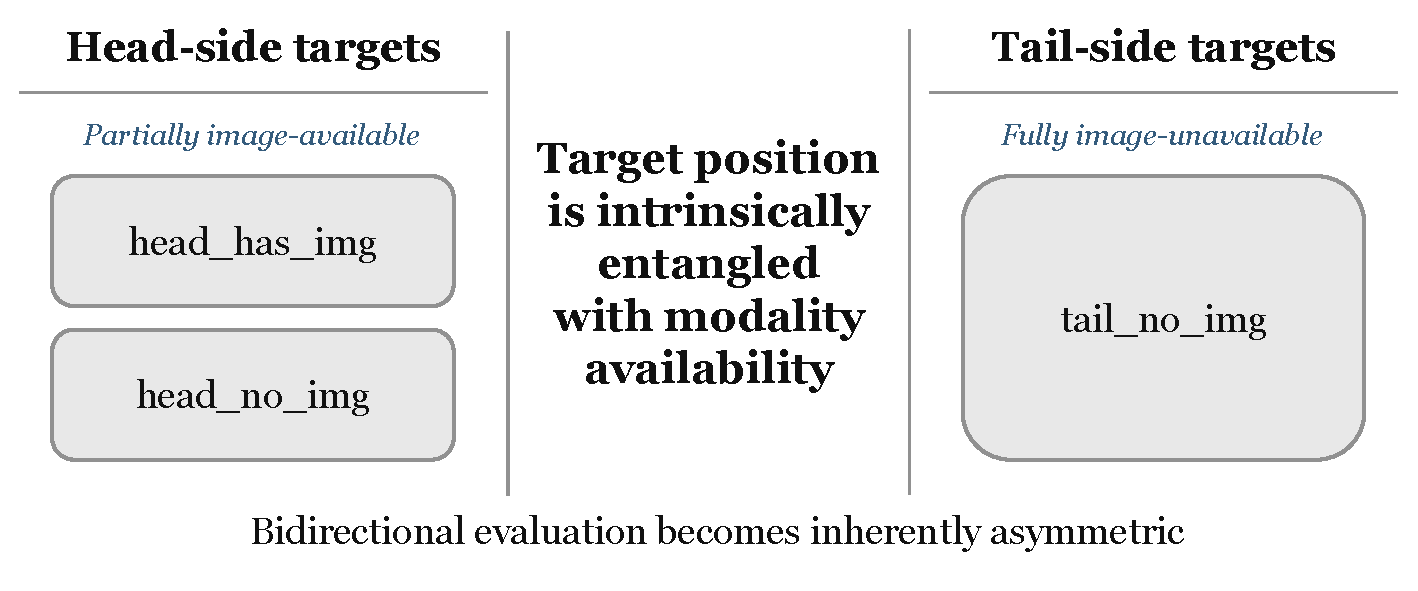
\includegraphics[width=0.8\\textwidth]{Figure1.pdf}
    \\caption{Protocol-defined target-side availability structure in OpenBG-IMG. At test time, head-side targets are only partially image-available, whereas tail-side targets are image-unavailable. This induces exactly three meaningful target-side regimes---\\texttt{head\\_has\\_img}, \\texttt{head\\_no\\_img}, and \\texttt{tail\\_no\\_img}---and explains why bidirectional evaluation is not symmetric in practice under the current protocol.}
    \\label{fig:protocol_asymmetry}
\\end{figure}

Figure~\\ref{fig:protocol_asymmetry} is therefore not just a conceptual illustration. It defines the target-side availability structure that later subgroup evaluation reuses directly, and it motivates the routing problem itself: when multimodal gain depends on protocol-shaped query conditions, activation should be query-selective rather than always-on.

\\subsection{Unified Training and Selection Protocol}
All base models are trained under a unified train/dev/test workflow. The development split is used for early stopping and checkpoint selection, and all final paper-facing metrics are reported on the test split. This separation prevents exploratory observations from leaking into final claims.

For each completed base model, the reported checkpoint is the \\texttt{best.ckpt} selected according to development performance. We do not compare arbitrary terminal checkpoints. The same checkpoint-selection principle is reused across official comparison, subgroup evaluation, relation-group evaluation, behavior summaries, and case interpretation so that all downstream analyses remain grounded in the same model instances.

Router training follows the same separation principle at the feature-label level: query-level gain labels and relation priors are constructed from development-side expert outcomes only, and the trained router is then applied to test-side query features without using test labels during training. In the current first-round routing study, multiple router families, gain margins \\(\\delta\\), and inference thresholds \\(\\tau\\) are scanned and the strongest learned settings are reported on the routing line. These scans should therefore be interpreted as routing-study model analysis rather than as a fully locked held-out hyperparameter-selection protocol.

\\subsection{Evaluation Protocol}
All formal comparisons use filtered ranking metrics on the test set, including MRR, Hits@1, Hits@3, and Hits@10. All main paper-stage comparisons use \\texttt{direction=both}, so both head prediction and tail prediction are included in evaluation.

Under this \\texttt{both} protocol, the target-side asymmetry of the current split becomes much more consequential for interpretation. The protocol is therefore not just a reporting choice; it is part of the reason the paper observes local multimodal gain alongside globally stronger structure-heavy performance.

Later subgroup and relation-level analyses are not separate ad hoc experiments. They reuse the same test split, the same filtered-ranking setup, and the same selected checkpoints, but restrict aggregation to subsets of queries or relations. In other words, they are protocol-consistent decompositions of the same underlying evaluation problem rather than parallel evaluation pipelines.

\\subsection{Protocol-Aware Subgroup Structure}
Because the current \\texttt{paper\\_split} is asymmetric, subgroup analysis must also be defined in a protocol-aware way. We therefore analyze only the three meaningful target-side regimes under the current test distribution:

\\begin{itemize}
    \\item \\texttt{head\\_has\\_img}
    \\item \\texttt{head\\_no\\_img}
    \\item \\texttt{tail\\_no\\_img}
\\end{itemize}

We do not define \\texttt{tail\\_has\\_img} for the final analysis because it does not meaningfully exist under the current test distribution. This is why the router is not solving an abstract symmetric MMKGC problem; it is making decisions under a specific three-regime protocol whose support is quantified in Table~\\ref{tab:protocol_test_regime_counts}.

This subgroup structure also defines the boundary of later claims. When we say that multimodal gain is strongest in \\texttt{head\\_has\\_img}, this is not a universal claim about head prediction or multimodal KGC in general. It is a protocol-specific interpretation under the current OpenBG-IMG setting.

\\subsection{Protocol-Aware Relation Analysis}
Relation-type analysis is conducted under the same protocol rather than under a separately constructed benchmark. We use a coarse grouping file that organizes relations into \\texttt{visual\\_relations}, \\texttt{weak\\_visual\\_relations}, and \\texttt{ambiguous\\_material\\_relations}.

All grouped and relation-level metrics are computed from the same selected paper-stage runs and the same filtered-ranking procedure. For relation-level interpretation, we apply a minimum-support filter of \\texttt{MIN20} so that extremely small-support relations do not dominate the narrative.

The purpose of this grouping is analytical rather than taxonomic. It is not intended to prove that visual relations as a whole are globally favorable to multimodal models. Instead, it is used to test whether multimodal gain is relation-dependent and whether that dependence supports a global or only local advantage. In the present paper, this matters because relation dependence is one reason a learned query-level router can outperform a shallow global rule.

\\subsection{Official Results vs Routing Results}
The paper contains two complementary evaluation dialects, and the distinction between them is a global rule rather than a presentational detail.

\\begin{table}[t]
\\centering
\\caption{Two evaluation dialects used in this paper. Rows from these two lines must not be compared as if they came from the same aggregation basis.}
\\label{tab:evaluation_dialects}
\\small
\\begin{tabular}{p{0.22\\textwidth}p{0.28\\textwidth}p{0.38\\textwidth}}
\\toprule
Dialect & Aggregation basis & Used for \\\\
\\midrule
Official model-comparison line & formal \\texttt{test\\_metrics.json} outputs & ranking the original seven-model family under the paper protocol \\\\
Routing line & query-level exported expert outcomes with recomputed aggregation & comparing Oracle, rule-based routing, learned routing, and fixed experts on a shared routing-compatible basis \\\\
\\bottomrule
\\end{tabular}
\\end{table}

The official model-comparison line is used for the seven-model comparison among \\texttt{Text-only}, \\texttt{Early Fusion}, \\texttt{Gate-only}, \\texttt{Residual-only}, \\texttt{Full Model}, \\texttt{ComplEx}, and \\texttt{TuckER}. The routing line is used because Oracle routing, rule-based routing, and learned routing all operate on query-level expert predictions; for fairness, fixed experts inside that comparison are also reported on the same query-level recomputed basis.

These two lines answer different questions and must not be mixed in the same table or in the same direct row-to-row comparison. The official line establishes the ranking of the original models under the paper protocol. The routing line establishes whether selective activation improves over fixed experts once all rows are placed on a shared routing-compatible basis.

\\subsection{Why Protocol Details Matter for the New Paper}
The protocol described above is not a neutral implementation detail. Under the current OpenBG-IMG setting, it creates a bounded-gain, query-dependent multimodal scenario rather than a generic symmetric MMKGC benchmark.

This is why the paper moves from gain-boundary analysis to gain-aware selective activation. The protocol does not merely contextualize the method; it creates the decision problem that the router is designed to solve.

\\section{Method: Gain-Threshold Routing for Selective Multimodal Activation}
\\subsection{Overview}
The method introduced in this section is motivated by one central observation: under the current OpenBG-IMG protocol, multimodal gain is conditional rather than globally reliable. We therefore recast the problem as \\textbf{gain-aware selective activation}: instead of building a larger always-on multimodal encoder, we decide at the query level whether multimodal fusion is worth activating.

The proposed framework is deliberately lightweight. It keeps the experts fixed, uses a small router on top of them, and attributes any resulting gain to selective activation rather than to added model capacity or a newly trained end-to-end multimodal architecture.

\\subsection{Problem Formulation}
For a query \\(q\\), we consider either tail prediction \\((h,r,?)\\) or head prediction \\((?,r,t)\\). Under the protocol-aware target-side regime structure defined in Section~3, the usefulness of multimodal fusion is not symmetric across queries.

The routing problem is therefore defined at the query level rather than at the candidate level: given a query \\(q\\), decide whether multimodal fusion is expected to provide sufficient gain over a stronger structural alternative, and activate the corresponding expert accordingly. In this formulation, \\(y(q)\\) denotes a gain-positive query label, \\(\\tau\\) denotes the routing threshold, and the goal is not to use multimodal evidence everywhere but to decide \\textbf{when multimodal evidence is worth using} under the current protocol.

\\subsection{Dual-Expert Gain-Threshold Routing}
\\paragraph{Fixed experts.}
We define two fixed experts:

\\begin{itemize}
    \\item \\textbf{Fusion expert:} \\texttt{Gate-only}
    \\item \\textbf{Structural expert:} \\texttt{Residual-only}
\\end{itemize}

This choice is deliberate rather than ad hoc. The pair gives the clearest within-family competition between relation-aware multimodal fusion and structure-heavy fallback, preserves diagnostic clarity, and provides an interpretable basis for selective routing.

\\paragraph{Why not route with \\texttt{Full Model}?}
Using \\texttt{Full Model} as the fusion-side routed expert would be tempting, but it would also blur the interpretation because \\texttt{Full Model} already contains an internal residual path. We therefore do not use it as the routed fusion expert in the first version of the method. Routing between \\texttt{Gate-only} and \\texttt{Residual-only} isolates expert selection from the internal branch competition already present in \\texttt{Full Model} and keeps the comparison interpretable as \\textbf{fusion versus structural fallback}.

\\paragraph{Query-level routing formulation.}
Let \\(s_f(q,e)\\) denote the score assigned to candidate entity \\(e\\) for query \\(q\\) by the fusion expert, and let \\(s_s(q,e)\\) denote the corresponding score from the structural expert. A router receives a query-level feature vector \\(x_q\\) and predicts the probability that fusion should be selected:

\\[
p(q)=P(y=1\\mid x_q).
\\]

We then apply hard routing with threshold \\(\\tau\\):

\\[
\\alpha(q)=\\mathbf{1}[p(q)>\\tau].
\\]

The final score is defined as

\\[
s_{\\text{final}}(q,e)=\\alpha(q)s_f(q,e)+(1-\\alpha(q))s_s(q,e).
\\]

This design keeps the experts fixed and places the method contribution on the selection rule itself. It is also better aligned with the current bounded-gain setting than soft blending everywhere, because the main question is whether fusion should be activated for the current query at all.

\\subsection{Gain Label Construction}
Router supervision is constructed per query, not per candidate entity. For each query \\(q\\), we compute the filtered rank of the correct target entity under the fusion expert and the structural expert, denoted by \\(\\mathrm{rank}_f(q)\\) and \\(\\mathrm{rank}_s(q)\\), respectively. All ranks are computed under the same filtered-ranking protocol as the final task evaluation.

We convert ranks into reciprocal ranks:

\\[
RR_f(q)=\\frac{1}{\\mathrm{rank}_f(q)}, \\qquad RR_s(q)=\\frac{1}{\\mathrm{rank}_s(q)}.
\\]

The gain difference is then defined as

\\[
\\Delta(q)=RR_f(q)-RR_s(q).
\\]

Using reciprocal-rank difference aligns the label with ranking improvement rather than with raw score magnitude. We define the binary gain label as

\\[
y(q)=\\mathbf{1}[\\Delta(q)>\\delta],
\\]

where \\(\\delta\\) is a gain margin controlling how conservative the definition of a gain-positive query is.

This label should not be interpreted as a semantic class of inherently multimodal-friendly queries. It only means that, under the current protocol and the current expert pair, the fusion expert yields sufficiently larger reciprocal-rank improvement than the structural expert for this specific query.

In the first-round routing study, we evaluate \\(\\delta\\in\\{0.00,0.01,0.02\\}\\). All gain labels are constructed from development-side expert outcomes only. Test labels are never used for router training, and relation priors are estimated strictly from train/dev-side information to avoid leakage.

\\subsection{Protocol-Aware Router Features}
The feature design follows one guiding principle: a useful router should not collapse into the shallow rule ``use fusion whenever images are available.'' We therefore combine protocol-aware condition features, modality-consistency features, and expert-confidence features.

\\begin{table}[t]
\\centering
\\caption{Router feature definitions in the \\texttt{FULL} setting.}
\\label{tab:router_feature_definitions}
\\small
\\begin{tabular}{p{0.20\\textwidth}p{0.12\\textwidth}p{0.36\\textwidth}p{0.22\\textwidth}}
\\toprule
Feature & Type & Definition & Source \\\\
\\midrule
\\texttt{direction} & categorical & query direction (head / tail) & current query \\\\
\\texttt{target\\_has\\_img} & binary & whether the target entity has image support & current query \\\\
\\texttt{target\\_regime} & categorical & \\texttt{head\\_has\\_img}, \\texttt{head\\_no\\_img}, or \\texttt{tail\\_no\\_img} & current query \\\\
\\texttt{relation\\_id} & categorical & relation identifier & current query \\\\
\\texttt{relation\\_gain\\_prior} & numeric & mean gain-oriented prior estimated for the relation & dev-side relation stats \\\\
\\texttt{relation\\_fusion\\_win\\_rate} & numeric & fraction of dev queries on which fusion beats structure for that relation & dev-side relation stats \\\\
\\texttt{relation\\_support} & numeric & support count for that relation in prior estimation & dev-side relation stats \\\\
\\texttt{relation\\_is\\_visual\\_prior} & binary & binary flag derived from the relation prior statistics & dev-side relation stats \\\\
\\texttt{text\\_img\\_cosine} & numeric & cosine similarity between text and image representations & modality cache / current query \\\\
\\texttt{img\\_is\\_missing\\_replaced} & binary & whether the image branch uses a missing-image replacement vector & modality cache / current query \\\\
\\texttt{fusion\\_margin} & numeric & top1--top2 score gap from \\texttt{Gate-only} & current query expert output \\\\
\\texttt{struct\\_margin} & numeric & top1--top2 score gap from \\texttt{Residual-only} & current query expert output \\\\
\\texttt{fusion\\_correct\\_score} & numeric & score of the correct target under \\texttt{Gate-only} & current query expert output \\\\
\\texttt{struct\\_correct\\_score} & numeric & score of the correct target under \\texttt{Residual-only} & current query expert output \\\\
\\texttt{delta\\_margin} & numeric & \\texttt{fusion\\_margin} $-$ \\texttt{struct\\_margin} & derived from expert outputs \\\\
\\bottomrule
\\end{tabular}
\\end{table}

Protocol-aware condition features describe the query under the current asymmetric protocol. Modality-consistency features describe whether the query appears to have coherent cross-modal evidence. Expert-confidence features describe whether one expert currently appears more trustworthy than the other, which is a stronger decision signal than raw image availability alone.

For learned routing, the current implementation uses the \\texttt{FULL} feature set by default. For ablation, we additionally define four nested feature subsets shown in Table~\\ref{tab:router_feature_sets}.

\\begin{table}[t]
\\centering
\\caption{Feature subsets used in ablation.}
\\label{tab:router_feature_sets}
\\small
\\begin{tabular}{p{0.10\\textwidth}p{0.78\\textwidth}}
\\toprule
Set & Features \\\\
\\midrule
\\texttt{F1} & \\texttt{target\\_has\\_img} \\\\
\\texttt{F2} & \\texttt{target\\_has\\_img}, \\texttt{direction}, \\texttt{relation\\_gain\\_prior} \\\\
\\texttt{F3} & \\texttt{F2} + \\texttt{text\\_img\\_cosine}, \\texttt{img\\_is\\_missing\\_replaced} \\\\
\\texttt{F4} & \\texttt{F3} + \\texttt{fusion\\_margin}, \\texttt{struct\\_margin}, \\texttt{delta\\_margin} \\\\
\\bottomrule
\\end{tabular}
\\end{table}

\\subsection{Router Baselines and Training}
We evaluate three router classes.

\\paragraph{Rule-based router.}
The rule-based baseline is defined as
\\[
\\text{route to fusion} \\iff \\texttt{target\\_has\\_img}=1 \\;\\text{and}\\; \\texttt{relation\\_gain\\_prior}>0.
\\]
It is intentionally shallow and serves as the strongest simple heuristic lower bound for learned routing.

\\paragraph{Logistic regression router.}
The first learned router is logistic regression. In the current implementation, it uses a sparse \\texttt{DictVectorizer} representation, \\texttt{solver=liblinear}, \\texttt{class\\_weight=balanced}, \\texttt{max\\_iter=2000}, and \\texttt{random\\_state=42}. Categorical features such as \\texttt{direction}, \\texttt{target\\_regime}, and \\texttt{relation\\_id} are string-encoded before vectorization. Missing values are mapped to \\(0.0\\) by construction.

\\paragraph{Gradient-boosted router.}
The second learned router is XGBoost. The current implementation uses \\texttt{n\\_estimators=300}, \\texttt{max\\_depth=4}, \\texttt{learning\\_rate=0.05}, \\texttt{subsample=0.8}, \\texttt{colsample\\_bytree=0.8}, \\texttt{reg\\_lambda=1.0}, \\texttt{objective=binary:logistic}, \\texttt{eval\\_metric=logloss}, \\texttt{random\\_state=42}, and \\texttt{n\\_jobs=1}. Class imbalance is handled through \\texttt{scale\\_pos\\_weight = N_{neg}/N_{pos}} computed from the current training labels.

\\paragraph{Training and selection protocol.}
All learned routers are trained on development-side query-level feature tables constructed from the fixed experts. The supervised target is the gain label defined above, and the trained router is then applied to test-side query features without observing test labels during training.

In the current first-round study, we train learned routers for multiple gain margins \\(\\delta\\) and then evaluate threshold scans over \\(\\tau\\in\\{0.1,0.3,0.5,0.7,0.9\\}\\). The strongest reported settings should therefore be interpreted as first-round empirical best settings within the routing study, not as the output of a fully locked held-out hyperparameter-selection protocol. This is why the present paper frames these routing results as a protocol-aware method demonstration rather than as a final hyperparameter-optimized benchmark submission.

\\subsection{Hard-Threshold Inference and Evaluation Dialects}
As an implementation consequence of the evaluation protocol defined in Section~3, all routing claims are made on the unified query-level recomputed line. Oracle routing, rule-based routing, and learned routing all require query-level exported expert outcomes, so fixed experts inside the routing comparison are also recomputed on that same basis for fairness.

These routing-compatible results must not be mixed with the official model-comparison line. Official model-family claims remain on the formal \\texttt{test\\_metrics.json} line, whereas routing claims are made only on the routing-compatible line.

\\subsection{Design Rationale and Scope}
The design is intentionally lightweight and interpretable. The experts are fixed rather than jointly optimized with the router, routing is performed at the query level rather than at the token or representation level, and hard-threshold routing is used instead of soft mixing. Together, these choices isolate the effect of selective activation itself.

The scope is also deliberately narrow. The current method is protocol-specific by construction: it is designed to show that, under the present OpenBG-IMG setting, bounded multimodal gain can be turned into a useful query-level decision problem. We do not claim that the same expert pair, feature space, or thresholding strategy should transfer unchanged to all MMKGC settings.

\\section{Experiments}
\\subsection{Experimental Setup}
All experiments in this section follow the protocol defined in Section~3, but the emphasis here is on execution and reporting. Base-model checkpoint selection uses development performance, and all final paper-facing base-model metrics are reported on the test split. For the official model-comparison line, results are reported as mean $\\pm$ standard deviation over three seeds whenever that aggregation is available.

\\begin{table}[t]
\\centering
\\caption{Experimental execution setup used in this paper.}
\\label{tab:experiment_setup}
\\small
\\begin{tabular}{p{0.34\\textwidth}p{0.58\\textwidth}}
\\toprule
Item & Value \\\\
\\midrule
Base-model checkpoint selection & \\texttt{best.ckpt} chosen on the development split \\\\
Official final reporting & filtered ranking on the test split with \\texttt{direction=both} \\\\
Official summary statistics & mean $\\pm$ standard deviation over three seeds \\\\
Routing training source & development-side query-level feature tables from fixed experts \\\\
Routing inference source & test-side query-level exported expert outcomes with unified recomputation \\\\
Gain-margin scan & $\\delta \\in \\{0.00, 0.01, 0.02\\}$ \\\\
Threshold scan & $\\tau \\in \\{0.1, 0.3, 0.5, 0.7, 0.9\\}$ \\\\
Meaningful target-side regimes & \\texttt{head\\_has\\_img}: 7{,}048 (35.24\\%), \\texttt{head\\_no\\_img}: 2{,}952 (14.76\\%), \\texttt{tail\\_no\\_img}: 10{,}000 (50.00\\%) \\\\
\\bottomrule
\\end{tabular}
\\end{table}

All results in this chapter belong to one of two evaluation lines: the official model-comparison line or the routing line. Direct comparisons are made only within line; cross-dialect numbers are not used as same-basis evidence in the experiments section.

\\subsection{Compared Methods and Evaluation Lines}
\\paragraph{Official model-comparison line.}
Table~\\ref{tab:compared_methods_official} summarizes the seven completed models compared on the official line.

\\begin{table}[t]
\\centering
\\caption{Methods compared on the official model-comparison line.}
\\label{tab:compared_methods_official}
\\small
\\begin{tabular}{p{0.20\\textwidth}p{0.22\\textwidth}p{0.46\\textwidth}}
\\toprule
Method & Family & Role in this paper \\\\
\\midrule
\\texttt{Text-only} & unimodal text & weak text reference inside the internal family \\\\
\\texttt{Early Fusion} & multimodal fusion & simple multimodal baseline \\\\
\\texttt{Gate-only} & multimodal fusion & fusion endpoint inside the internal family \\\\
\\texttt{Residual-only} & structure-heavy hybrid & strongest fixed internal reference \\\\
\\texttt{Full Model} & multimodal + residual hybrid & strongest internal multimodal variant \\\\
\\texttt{ComplEx} & classical structural & competitive external structural baseline \\\\
\\texttt{TuckER} & classical structural & retained classical reference under the current split \\\\
\\bottomrule
\\end{tabular}
\\end{table}

\\paragraph{Routing line.}
Table~\\ref{tab:compared_methods_routing} summarizes the direct routing-line comparison set. The router is trained on development-side query-level features and evaluated on test-side query-level exported expert outcomes.

\\begin{table}[t]
\\centering
\\caption{Methods compared directly on the routing line.}
\\label{tab:compared_methods_routing}
\\small
\\begin{tabular}{p{0.22\\textwidth}p{0.22\\textwidth}p{0.44\\textwidth}}
\\toprule
Method & Type & Role in this paper \\\\
\\midrule
\\texttt{Gate-only} & fixed expert & fusion expert on the routing-compatible basis \\\\
\\texttt{Residual-only} & fixed expert & structural expert on the routing-compatible basis \\\\
Rule-based & heuristic router & shallow protocol-aware lower bound \\\\
Logistic routing & learned router & lightweight linear decision boundary \\\\
XGBoost routing & learned router & nonlinear learned router and strongest learned setting \\\\
Oracle routing & upper-bound selector & routing headroom reference \\\\
\\bottomrule
\\end{tabular}
\\end{table}

\\texttt{Full Model} remains an official-line baseline and is discussed elsewhere in the paper, but it is not a direct row in the routing-line comparisons reported below.

\\subsection{Official Main Results}
\\paragraph{Seven-model comparison under the official line.}
Table~\\ref{tab:official_main_results} reports the official seven-model comparison under the formal paper protocol. The main descriptive result is clear: \\texttt{Residual-only} is strongest overall at \\texttt{0.2930 $\\pm$ 0.0008} MRR, \\texttt{ComplEx} is second at \\texttt{0.2588 $\\pm$ 0.0018}, and \\texttt{Full Model} is the strongest multimodal variant inside the internal family at \\texttt{0.2100 $\\pm$ 0.0097}. \\texttt{TuckER} is retained as a classical structural reference, but it does not emerge as competitive under the current split and protocol.

\\begin{table}[t]
\\centering
\\caption{Overall test performance under the unified OpenBG-IMG protocol with filtered ranking, \\texttt{direction=both}, and three-seed reporting.}
\\label{tab:official_main_results}
\\small
\\setlength{\\tabcolsep}{5pt}
\\begin{tabular}{lcccc}
\\toprule
Model & MRR & Hits@1 & Hits@3 & Hits@10 \\\\
\\midrule
\\texttt{Residual-only} & 0.2930 $\\pm$ 0.0008 & 0.2328 $\\pm$ 0.0003 & 0.3306 $\\pm$ 0.0021 & 0.4031 $\\pm$ 0.0017 \\\\
\\texttt{ComplEx} & 0.2588 $\\pm$ 0.0018 & 0.1920 $\\pm$ 0.0026 & 0.2946 $\\pm$ 0.0012 & 0.3871 $\\pm$ 0.0014 \\\\
\\texttt{Full Model} & 0.2100 $\\pm$ 0.0097 & 0.1167 $\\pm$ 0.0107 & 0.2658 $\\pm$ 0.0131 & 0.3794 $\\pm$ 0.0116 \\\\
\\texttt{Gate-only} & 0.1739 $\\pm$ 0.0044 & 0.0946 $\\pm$ 0.0108 & 0.2113 $\\pm$ 0.0030 & 0.3261 $\\pm$ 0.0010 \\\\
\\texttt{Early Fusion} & 0.1666 $\\pm$ 0.0013 & 0.0905 $\\pm$ 0.0008 & 0.1998 $\\pm$ 0.0034 & 0.3155 $\\pm$ 0.0022 \\\\
\\texttt{Text-only} & 0.1261 $\\pm$ 0.0043 & 0.0524 $\\pm$ 0.0050 & 0.1499 $\\pm$ 0.0036 & 0.2761 $\\pm$ 0.0046 \\\\
\\texttt{TuckER} & 0.0890 $\\pm$ 0.0024 & 0.0360 $\\pm$ 0.0019 & 0.1054 $\\pm$ 0.0042 & 0.1892 $\\pm$ 0.0012 \\\\
\\bottomrule
\\end{tabular}
\\end{table}

\\paragraph{Interpretation.}
The official line therefore establishes the paper's central tension: the strongest fixed model is structure-heavy, yet multimodal modeling still matters within the multimodal family because \\texttt{Full Model} consistently outperforms \\texttt{Gate-only}, \\texttt{Early Fusion}, and \\texttt{Text-only}. The reported standard deviations are small for \\texttt{Residual-only} and \\texttt{ComplEx} and larger for \\texttt{Full Model}, so we treat the three-seed means and standard deviations as descriptive stability evidence rather than as formal significance claims. This pattern motivates selective activation rather than a claim of global multimodal superiority.

\\subsection{Routing Results Under the Unified Query-Level Line}
Table~\\ref{tab:routing_results} reports the routing comparison under the unified query-level recomputed line. Within this line, the strongest learned router is XGBoost with $\\delta=0.01$ and $\\tau=0.7$, reaching \\texttt{0.3160} MRR and improving over both the fixed \\texttt{Residual-only} expert (\\texttt{0.2930}) and the rule-based router (\\texttt{0.2939}). Oracle routing reaches \\texttt{0.3337}, indicating that additional routing headroom still remains.

\\begin{table}[t]
    \\centering
    \\caption{Main routing-line comparison on the unified query-level recomputed basis. Direct comparisons in this table are restricted to the routing-compatible line.}
    \\label{tab:routing_results}
    \\small
    \\begin{tabular}{lcccc}
        \\toprule
        Method & $\\delta$ & $\\tau$ & MRR & Fusion coverage \\\\
        \\midrule
        \\texttt{Gate-only} (fixed expert) & -- & -- & 0.1688 & -- \\\\
        \\texttt{Residual-only} (fixed expert) & -- & -- & 0.2930 & -- \\\\
        Rule-based routing & 0.01 & 0.5 & 0.2939 & 0.0187 \\\\
        Logistic routing & 0.01 & 0.7 & 0.3111 & 0.1788 \\\\
        XGBoost routing & 0.01 & 0.7 & 0.3160 & 0.1848 \\\\
        Oracle routing & -- & -- & 0.3337 & 0.4843 \\\\
        \\bottomrule
    \\end{tabular}
\\end{table}

These routing results support the method claim cleanly within line. The rule-based router yields only a negligible improvement over the fixed structural expert, whereas learned routing produces a clear gain. This indicates that the gain boundary cannot be reduced to a single heuristic such as ``use fusion whenever images are available'' and is better understood as a richer query-level selective-activation problem.

\\subsection{Subgroup Evaluation}
Aggregate metrics alone do not explain why the official and routing results look the way they do, so we next decompose performance over the same three meaningful target-side regimes: \\texttt{head\\_has\\_img}, \\texttt{head\\_no\\_img}, and \\texttt{tail\\_no\\_img}. Table~\\ref{tab:subgroup_support} reports the subgroup support counts that determine how strongly each regime can influence the overall metric.

\\begin{table}[t]
\\centering
\\caption{Support of the three meaningful target-side regimes under the current test distribution.}
\\label{tab:subgroup_support}
\\small
\\begin{tabular}{lcc}
\\toprule
Regime & Queries & Proportion \\\\
\\midrule
\\texttt{head\\_has\\_img} & 7{,}048 & 35.24\\% \\\\
\\texttt{head\\_no\\_img} & 2{,}952 & 14.76\\% \\\\
\\texttt{tail\\_no\\_img} & 10{,}000 & 50.00\\% \\\\
\\bottomrule
\\end{tabular}
\\end{table}

Table~\\ref{tab:subgroup_results} reports subgroup MRR by target-side image availability for the three core diagnostic variants---\\texttt{Gate-only}, \\texttt{Full Model}, and \\texttt{Residual-only}. The resulting pattern is not uniform across regimes. In \\texttt{head\\_has\\_img}, the ordering becomes \\texttt{Gate-only > Full Model > Residual-only}, identifying the clearest multimodal-favorable regime under the current protocol. In \\texttt{head\\_no\\_img}, the ordering becomes \\texttt{Full Model > Gate-only > Residual-only}, indicating that the complete model remains more stable than pure gated fusion when image support is absent on the head side. In \\texttt{tail\\_no\\_img}, however, \\texttt{Residual-only} remains decisively strongest. Because \\texttt{tail\\_no\\_img} accounts for 50\\% of all bidirectional queries, this regime exerts the strongest pull on the aggregate result.

\\begin{table}[t]
\\centering
\\caption{Subgroup MRR by target-side image availability under the current protocol. All cells report mean $\\pm$ standard deviation over seeds 1, 2, and 3.}
\\label{tab:subgroup_results}
\\small
\\setlength{\\tabcolsep}{5pt}
\\begin{tabular}{lccc}
\\toprule
Model & \\texttt{head\\_has\\_img} & \\texttt{head\\_no\\_img} & \\texttt{tail\\_no\\_img} \\\\
\\midrule
\\texttt{Residual-only} & 0.0017 $\\pm$ 0.0001 & 0.0055 $\\pm$ 0.0003 & 0.5832 $\\pm$ 0.0015 \\\\
\\texttt{Full Model} & 0.0069 $\\pm$ 0.0009 & 0.0119 $\\pm$ 0.0014 & 0.4116 $\\pm$ 0.0193 \\\\
\\texttt{Gate-only} & 0.0125 $\\pm$ 0.0004 & 0.0108 $\\pm$ 0.0014 & 0.3359 $\\pm$ 0.0087 \\\\
\\bottomrule
\\end{tabular}
\\end{table}

The strongest learned router also follows a selective subgroup pattern rather than a global one. Table~\\ref{tab:subgroup_router_behavior} reports the subgroup MRR and fusion coverage of the best learned setting (\\texttt{xgb}, $\\delta=0.01$, $\\tau=0.7$). Fusion is retained most cautiously in the structure-favorable regimes and remains available where local multimodal gain is more plausible.

\\begin{table}[t]
\\centering
\\caption{Subgroup behavior of the strongest learned router (XGBoost, $\\delta=0.01$, $\\tau=0.7$).}
\\label{tab:subgroup_router_behavior}
\\small
\\begin{tabular}{lcc}
\\toprule
Regime & MRR & Fusion coverage \\\\
\\midrule
\\texttt{head\\_has\\_img} & 0.0116 & 0.1501 \\\\
\\texttt{head\\_no\\_img} & 0.0125 & 0.1059 \\\\
\\texttt{tail\\_no\\_img} & 0.6200 & 0.2326 \\\\
\\bottomrule
\\end{tabular}
\\end{table}

Taken together, the subgroup evidence shows how the aggregate routing gain is produced. The router is not behaving randomly; it is adapting differently across regimes whose supports are themselves highly uneven. This is exactly the pattern expected if the learned decision boundary is capturing protocol-aware gain structure rather than a shallow shortcut.

\\subsection{Threshold Scan}
Table~\\ref{tab:threshold_scan_summary} summarizes the threshold scan for the learned routers at $\\delta=0.01$. For both logistic regression and XGBoost, MRR rises as the router becomes more conservative, peaks at $\\tau=0.7$, and then flattens or declines slightly at $\\tau=0.9$. At the same time, fusion coverage decreases monotonically, while gain precision increases monotonically.

\\begin{table}[t]
\\centering
\\caption{Threshold scan summary at $\\delta=0.01$.}
\\label{tab:threshold_scan_summary}
\\small
\\begin{tabular}{cccccc}
\\toprule
$\\tau$ & Logistic MRR & Logistic coverage & XGBoost MRR & XGBoost coverage & XGBoost gain precision \\\\
\\midrule
0.1 & 0.2338 & 0.6136 & 0.2514 & 0.4831 & 0.3270 \\\\
0.3 & 0.2817 & 0.3852 & 0.2921 & 0.3334 & 0.4518 \\\\
0.5 & 0.3013 & 0.2681 & 0.3084 & 0.2524 & 0.5548 \\\\
0.7 & 0.3111 & 0.1788 & 0.3160 & 0.1848 & 0.6696 \\\\
0.9 & 0.3101 & 0.0911 & 0.3142 & 0.0962 & 0.8460 \\\\
\\bottomrule
\\end{tabular}
\\end{table}

This scan supports the selective-activation hypothesis directly. Performance does not improve by activating fusion more aggressively; it improves by becoming selective enough to suppress low-value fusion while still preserving some useful local multimodal cases. The best setting therefore corresponds to a balanced threshold rather than to maximum fusion usage.

\\subsection{Feature Ablation}
To test whether routing success comes only from shallow image-availability cues, we evaluate four incremental feature sets, from the minimal image-availability signal (\\texttt{F1}) to the full protocol-aware, modality-consistency, and expert-confidence setting (\\texttt{F4}). Table~\\ref{tab:feature_ablation} reports the resulting overall MRR values.

\\begin{table}[t]
\\centering
\\caption{Feature ablation for learned routers at $\\delta=0.01$ and $\\tau=0.5$.}
\\label{tab:feature_ablation}
\\small
\\begin{tabular}{lcccc}
\\toprule
Model & \\texttt{F1} & \\texttt{F2} & \\texttt{F3} & \\texttt{F4} \\\\
\\midrule
Logistic & 0.1651 & 0.2333 & 0.2333 & 0.2501 \\\\
XGBoost & 0.1651 & 0.2306 & 0.2303 & 0.2556 \\\\
\\bottomrule
\\end{tabular}
\\end{table}

The hierarchy is clear. Image availability alone is insufficient, because \\texttt{F1} performs poorly for both models. Protocol-aware condition features are central, as shown by the large jump from \\texttt{F1} to \\texttt{F2}. The final jump from \\texttt{F3} to \\texttt{F4} shows that expert-confidence features complete the decision boundary and provide the strongest additional gain.

\\subsection{Relation-Group Evaluation}
Relation-group evidence is retained as supporting analysis rather than as a second main-result line. Its role is to test whether relation characteristics matter for bounded multimodal gain and to show why a single coarse heuristic is insufficient.

Table~\\ref{tab:relation_grouped} reports the grouped relation-type results. The same ordering appears in every coarse relation group: \\texttt{Residual-only} is strongest, \\texttt{Full Model} is second, and \\texttt{Gate-only} is third. These results show that relation dependence is real, but still bounded; they do not support a claim that visual relations as a whole become globally favorable to multimodal models.

\\begin{table}[t]
\\centering
\\caption{Relation-type grouped MRR under the unified OpenBG-IMG protocol. All cells report mean $\\pm$ standard deviation over seeds 1, 2, and 3.}
\\label{tab:relation_grouped}
\\small
\\setlength{\\tabcolsep}{5pt}
\\begin{tabular}{lccc}
\\toprule
Model & \\texttt{visual\\_relations} & \\texttt{weak\\_visual\\_relations} & \\texttt{ambiguous\\_material\\_relations} \\\\
\\midrule
\\texttt{Residual-only} & 0.2691 $\\pm$ 0.0011 & 0.3197 $\\pm$ 0.0010 & 0.2842 $\\pm$ 0.0028 \\\\
\\texttt{Full Model} & 0.1826 $\\pm$ 0.0071 & 0.2252 $\\pm$ 0.0154 & 0.1948 $\\pm$ 0.0201 \\\\
\\texttt{Gate-only} & 0.1350 $\\pm$ 0.0068 & 0.2194 $\\pm$ 0.0073 & 0.1337 $\\pm$ 0.0083 \\\\
\\bottomrule
\\end{tabular}
\\end{table}

With the \\texttt{MIN20} support filter at the relation level, \\texttt{Full Model} still outperforms \\texttt{Gate-only} on most retained relations, but surpasses \\texttt{Residual-only} on only a minority of them. The retained support details remain in the supporting relation-level files and are not restated here so that this section stays focused on grouped tendencies rather than becoming a second primary result block.

\\subsection{Overall Experimental Summary}
Under the official line, the core tension remains unchanged: \\texttt{Residual-only} is the strongest fixed model overall, while \\texttt{Full Model} is the strongest multimodal variant inside the internal family.

Under the routing line, selective activation is effective: the best learned router is XGBoost with $\\delta=0.01$ and $\\tau=0.7$, and it improves over both the fixed structural expert and the rule-based router on the shared routing-compatible basis.

Subgroup, threshold-scan, feature-ablation, and relation-group evidence all support the same interpretation: multimodal gain in the current protocol is local, protocol-shaped, and query-dependent, which is why a selective router can exploit it more effectively than a shallow global heuristic.

\\section{Analysis and Discussion}
\\subsection{Overview}
The discussion begins from two result layers that should be kept distinct. Under the official model-comparison line, \\texttt{Residual-only} remains the strongest fixed model overall, while \\texttt{Full Model} remains the strongest multimodal variant inside the internal family. Under the routing-compatible line, the best learned router is XGBoost with $\\delta=0.01$ and $\\tau=0.7$, and it improves over the fixed-expert baselines and the rule-based router on that shared basis.

Taken together, these two layers suggest a more precise interpretation of the problem. The main issue is not that multimodal evidence has no value, but that its usefulness is conditional and requires a mechanism that activates it when it is likely to help and suppresses it when stronger structural fallback is more reliable.

\\subsection{Why Selective Activation Works Under the Current Protocol}
The current results indicate that multimodal gain is heterogeneous across the evaluation space rather than globally uniform. Subgroup evidence shows that the clearest favorable regime appears in \\texttt{head\\_has\\_img}, whereas the globally dominant \\texttt{tail\\_no\\_img} regime remains strongly structure-favorable. Relation-group results point in the same direction: relation dependence is real, but bounded, and does not overturn the stronger structural tendency at the grouped level.

Under such a protocol-shaped heterogeneous setting, routing becomes a natural formulation. An always-on model must compromise across queries with different gain structures, whereas a router can preserve the fusion expert for one subset of queries and rely on structural fallback for another. In this sense, bounded gain is naturally re-expressed as a query-level expert-selection problem rather than as a universal architecture problem~\\cite{zhao2022mose,liang2023hrgat,jacobs1991adaptive,shazeer2017outrageously}.

The gap between \\texttt{Full Model} and the learned router is especially informative. This gap should not be read as evidence that the multimodal branch inside \\texttt{Full Model} learned nothing useful. A more plausible interpretation is that the current protocol encourages a global compromise inside one shared representation: multimodal fusion remains useful locally, but the final model must still accommodate a large structure-favorable region. The current results are therefore more consistent with a \\textit{compromise limitation} than with multimodal uselessness.

By contrast, the router does not need to learn one globally balanced representation. It can partition queries directly and preserve fusion where local gain is plausible while defaulting to structural fallback elsewhere. This is why selective activation works naturally under the current protocol.

\\subsection{Why Learned Routing Beats Rule-Based Heuristics}
A simple reading of the protocol might suggest an easy rule: use fusion when images are available and avoid it when they are not. The experiments show that this intuition is incomplete. The rule-based router improves only negligibly over the fixed structural expert, whereas learned routing yields a clear gain.

This difference implies that the gain boundary is richer than a single image-availability flag. Relation context matters, subgroup conditions matter, and expert-confidence signals matter as well. The decision problem is therefore not ``has image or not'' but whether the current query is likely to benefit sufficiently from fusion relative to the structural fallback.

The feature-ablation results reinforce this interpretation. \\texttt{F1} performs poorly, which rules out a pure image-availability explanation. The jump to \\texttt{F2} shows that protocol-aware condition features are central, and the jump from \\texttt{F3} to \\texttt{F4} shows that expert-confidence signals complete the decision boundary. The stronger performance of XGBoost over logistic regression is consistent with the same conclusion: the routing boundary is interaction-rich rather than purely linear.

\\subsection{How the New Results Reposition \\texttt{Gate-only}, \\texttt{Residual-only}, and \\texttt{Full Model}}
\\paragraph{\\texttt{Gate-only} is locally useful, not globally reliable.}
\\texttt{Gate-only} should not be positioned as a failed model. It remains the clearest fusion endpoint in the internal family and performs best in the most multimodal-favorable subgroup, namely \\texttt{head\\_has\\_img}. In the new paper, its importance is not global dominance but diagnostic clarity: it is useful enough to serve as the fusion expert inside a selective system.

\\paragraph{\\texttt{Residual-only} is more than an ablation baseline.}
\\texttt{Residual-only} should also not be treated as a mere ablation. It is the strongest fixed structural reference inside the internal family and functions as the reliable fallback expert around which the routing problem is organized. Its strength is exactly why selective activation becomes necessary under the current protocol.

\\paragraph{\\texttt{Full Model} remains analytically important even if it is not the final winner.}
\\texttt{Full Model} remains a key diagnostic reference even though it is not the final winner. Its value is that it demonstrates the limitation of always-on multimodal enhancement under the current protocol: even when fusion and structural compensation are integrated inside one richer model, protocol-shaped gain heterogeneity still prevents that always-on design from becoming globally optimal. In this sense, \\texttt{Full Model} remains the main bridge between the earlier bounded-gain analysis and the current routing formulation.

\\subsection{What Relation-Group Evidence Still Contributes}
Relation-group evidence does not show that coarse semantic grouping has already solved the routing problem, nor does it show that visual relations as a whole become globally favorable to multimodal models.

What it does show is still useful: multimodal benefit is not random, but the decision boundary is too fine-grained and too interaction-dependent to be handled by one coarse grouped rule. For that reason, relation-group analysis remains a supporting bridge for the selective-activation story rather than a second main result line.

\\subsection{What the New Results Do Not Prove}
The strongest claim supported by this paper is narrow and deliberate: \\textbf{selective activation is effective under the current OpenBG-IMG protocol}. Several stronger claims are not supported and should be avoided.

First, the results do not show that multimodal fusion is globally superior to structural modeling in general. Strong structural fallback remains indispensable, and the strongest fixed model is still structure-heavy.

Second, the results do not show that the current gain-threshold router is the final or universally best solution for bounded multimodal gain. The present method is intentionally lightweight and controlled.

Third, the results do not show that the same expert pair, thresholding strategy, or feature design transfers unchanged to other MMKGC benchmarks or to different OpenBG-IMG splits. The contribution is protocol-aware by construction.

These limits are not weaknesses to hide. They are part of the paper's credibility. The strongest framing of the current work is therefore a careful, protocol-grounded demonstration rather than a universal multimodal claim.

\\subsection{Broader Implications}
First, protocol-aware evaluation matters. Target position, modality availability, and relation structure can jointly determine whether multimodal information appears useful at all.

Second, strong structural competitors remain essential interpretive anchors. Without them, the bounded-gain story would be much less informative.

Third, the current results suggest that deciding \\textbf{when} to trust multimodal evidence can be as important as deciding \\textbf{how} to fuse it~\\cite{jacobs1991adaptive,jordan1994hierarchical,shazeer2017outrageously}.

\\section{Limitations}
\\subsection{Protocol Specificity}
The most important limitation of this study is that its strongest claims are \\textbf{protocol-aware rather than universal}. The central findings are derived under the current OpenBG-IMG \\texttt{paper\\_split}, unified train/dev/test workflow, filtered ranking, and \\texttt{direction=both} evaluation. Under a different split, a different modality distribution, or a more symmetric target-side condition, the relative strength of multimodal fusion, structural compensation, and selective routing could change.

This limitation is not incidental. The entire argument of the paper begins from the observation that the current protocol creates a meaningful but asymmetric missing-visual setting. As a result, the paper should not claim that bounded multimodal gain or gain-threshold routing has exactly the same form in all MMKGC settings. The strongest defensible statement is narrower: under the present OpenBG-IMG protocol, multimodal gain is conditional and query-dependent, and selective activation is an effective way to exploit it.

\\subsection{Entanglement Between Target Position and Modality Availability}
A second limitation is the entanglement between target position and image availability. In the current test distribution, head-side targets can still be image-supported, whereas tail-side targets are effectively \\texttt{no\\_img}. This asymmetry is analytically useful because it reveals the gain boundary clearly, but it also restricts generalization.

In particular, the conclusion that multimodal gain is strongest in \\texttt{head\\_has\\_img} should not be read as a universal superiority of head-side prediction or as a claim that tail-side prediction is inherently structure-only in multimodal KGC. It is a finding tied to the present protocol, where target position and modality availability are coupled. A more symmetric benchmark could lead to a different distribution of local multimodal benefit.

\\subsection{Fixed-Expert Routing Scope}
The proposed method is intentionally lightweight and controlled. We fix two experts - \\texttt{Gate-only} and \\texttt{Residual-only} - and learn a query-level router on top of them. This is a strength for interpretability, because it isolates the contribution of selective activation itself. However, it is also a limitation.

Other possibilities remain open, including routing with different expert families, incorporating \\texttt{ComplEx} or other structural references, using soft rather than hard routing, adopting end-to-end co-adaptive training of experts and router, and moving from query-level to representation-level routing.

The present paper does not attempt to cover these alternatives. Its goal is narrower: to show that bounded multimodal gain can already be operationalized effectively with a simple, interpretable routing framework.

\\subsection{Evaluation-Dialect Separation}
Another limitation is that the paper necessarily relies on two complementary evaluation dialects.

The official seven-model comparison uses the paper-facing \\texttt{test\\_metrics.json} aggregation line. The routing experiments use a unified query-level recomputed line, because Oracle, rule-based routing, and learned routing all depend on query-level exported expert outcomes. This separation is methodologically justified and necessary for fairness inside the routing experiments, but it also introduces additional complexity into presentation and interpretation.

Although the paper makes this distinction explicit, readers must still interpret some tables with care. In particular, the fixed experts in the routing comparison are not simply copied from the official main-result table; they are recomputed under the routing-compatible line. This is the correct choice for internal consistency, but it also means the paper cannot be read as if every number came from one single aggregation pipeline.

\\subsection{Coarseness of Relation-Group and Feature Design}
The relation-group analysis in this paper is deliberately coarse and analysis-oriented. The groups such as \\texttt{visual\\_relations}, \\texttt{weak\\_visual\\_relations}, and \\texttt{ambiguous\\_material\\_relations} are useful for testing whether multimodal gain varies with broad relation characteristics, but they do not define a complete semantic ontology of relations. Likewise, the router feature sets are designed to test protocol-aware selective activation in a controlled way, not to exhaust every possible feature family.

As a result, the current paper should not be interpreted as offering a final taxonomy of multimodal-favorable relation types or a complete characterization of all useful router features. Instead, it provides a first operational decomposition showing that target regime, relation priors, and expert-confidence signals already contain enough information to support effective selective activation under the current protocol.

\\subsection{No Claim of Universal Multimodal Superiority}
Finally, the present work does not claim that multimodal fusion is globally superior to structural modeling in MMKGC. In fact, one of the paper's central empirical findings is the opposite: under the current protocol, strong structural fallback remains indispensable, and the strongest fixed model is still structure-heavy.

This is a limitation in the sense that the paper does not deliver a universally dominant multimodal architecture. But it is also part of the paper's honesty and positioning. The contribution is not to ``win MMKGC'' in the most general sense. It is to identify a bounded-gain regime clearly and then show that once this regime is treated as a routing problem, selective activation can outperform always-on multimodal use under the present setting.

\\section{Conclusion}
This paper revisits multimodal knowledge graph completion on OpenBG-IMG under a more precise question than the standard ``does multimodal information help?'' framing. Under the current protocol, the answer is not a simple yes or no. Multimodal information is useful, but its usefulness is not globally uniform. It depends on target position, image availability, relation context, and the competition between multimodal fusion and stronger structural compensation.

The first contribution of the paper is analytical. Through protocol-aware subgroup analysis, relation-group evaluation, and behavior interpretation, we show that multimodal gain in the current OpenBG-IMG setting is \\textbf{real but bounded}. The clearest multimodal-favorable regime appears in \\texttt{head\\_has\\_img}, while the globally dominant \\texttt{tail\\_no\\_img} regime remains more favorable to structure-heavy modeling. Relation-group evidence further shows that multimodal benefit is relation-dependent but not strong enough to overturn structural dominance at the grouped level. Behavior analysis explains this pattern internally: the fusion path remains meaningful and adaptive, but the final system preference is still residual-dominant, especially when image support is weak.

The second contribution is methodological. Rather than stopping at the conclusion that multimodal gain is bounded, we reformulate this bounded-gain structure as a \\textbf{query-level selective activation problem}. The proposed gain-threshold routing framework uses \\texttt{Gate-only} as a fusion expert, \\texttt{Residual-only} as a structural expert, and a lightweight router to decide whether multimodal activation is worth using for the current query. Under the unified routing line, the best learned router is the XGBoost setting with $\\delta=0.01$ and $\\tau=0.7$, reaching \\texttt{0.3160} MRR and outperforming the strongest fixed expert, the rule-based router, and the original always-on \\texttt{Full Model}, while still leaving a gap to Oracle routing.

The significance of this result should be interpreted carefully. The paper does not claim that multimodal fusion is universally superior to structural modeling, nor does it claim that the present gain-threshold router is the final solution to MMKGC under incomplete visual support. Instead, the paper makes a more controlled and more defensible claim: under the current OpenBG-IMG protocol, multimodal gain is conditional rather than globally reliable, and once this condition-dependent structure is made explicit, selective activation can use multimodal evidence more effectively than always-on fusion.

In this sense, the contribution of the paper is not a globally dominant multimodal architecture, but a protocol-aware transition from \\textbf{gain-boundary analysis} to \\textbf{gain-aware selective activation}. We show not only when multimodal information helps and why that help remains bounded, but also how this bounded-gain structure can be turned into an operational routing mechanism. We hope this perspective encourages future MMKGC research to focus not only on how to fuse modalities more richly, but also on when multimodal evidence should be trusted at all under heterogeneous modality conditions.

\\bibliographystyle{plain}
\\bibliography{references}

\\end{document}
